\chapter{RESULTS AND DISCUSSIONS}
\label{ch:results}

\section{Introduction}
This chapter defines and explores the deliverables and objectives following their particular goals. This chapter extensively examines various aspects of the Alunan mobile application development process, including detailed descriptions of system requirements, user personas, storyboard creation, flowcharts, use case diagrams, database configurations, and the evolution of designs from low-fidelity to high-fidelity.

\section{Identification of System Requirements}
The process of identifying system requirements is comprehensive, requiring the collection, analysis, and documentation of the constraints and demands of a system or application \parencite{mokos20}. Generally, this process starts with stakeholder engagement to gain insight into the business objectives. Subsequently, requirements are obtained through workshops, surveys, and interviews. The examination of these requirements entails the recognition of connections, priorities, and possible conflicts; documentation serves to guarantee clear communication and consistency among the parties involved. Furthermore, the incorporation of validation and verification mechanisms serves to guarantee that the specified requirements precisely mirror the intended functionalities and limitations of the system. \\

The creation of system requirements is critical to the achievement of project objectives, as they provide the fundamental structure that guides the entirety of the development process. They offer designers, developers, and testers a strategic plan that directs their efforts toward developing a solution that satisfies the requirements of stakeholders. Incomplete or ambiguous requirements may necessitate expensive iterations of validation testing and design modifications in later stages. The unresolved difficulty of validating and refining system requirements early on emphasizes the significance of system requirements throughout the development process. \textcite{mokos20} stated that efficient and precisely defined requirements minimize the likelihood of costly rework or project failure, and promote clear communication among project teams. In simple terms, comprehensive system requirements increase the probability of successfully implementing a solution that fulfills the demands of stakeholders, accomplishes organizational goals, and provides value.

\subsection{System Requirements}
System requirements, as elucidated by \textcite{mokos20}, delineate the essential conditions and functionalities that a system must possess to meet the objectives and expectations of stakeholders. They function as a strategic plan that directs the development process by defining the intended functionalities, standards for performance, and limitations. Although frequently expressed in informal terms, system requirements may contain uncertainties, which calls for their formalization to achieve clarity and accuracy. \\

Addressing the development of the Alunan mobile application, this section provides a comprehensive overview of the system's requirements. Based on user expectations, system requirements are the capabilities that the system might be required to have The generation of potential solutions to a problem begins with the creative processes of ideation and brainstorming. By employing judgment and deduction, an extensive inventory of suggestions can be generated, a portion of which might even surpass the original ideas in terms of originality or unconventionality.

\begin{enumerate}[A.]
    \item \textbf{Functional Requirements and Non-Functional Requirements} \\ Functional requirements are the features or functions that developers must implement for users to complete their tasks. Meanwhile, non-functional requirements specify the attributes, characteristics, and constraints that govern the overall behavior, usability, and performance of a system, beyond its functional capabilities. These tasks should correspond to the problem statement presented in Chapter 1. Tables 4.1 and 4.2 show the functional and non-functional requirements for the Alunan mobile application. \\
    
    \begin{table}[htb]
        \caption{List of Functional Requirements for the Alunan Mobile Application}
        \label{tab:mytable}
        \centering
        \begin{tabular}{|p{7.5cm}|p{9.5cm}|}
        \hline
        \multicolumn{1}{|c|}{\textbf{Functional Requirements}} & 
        \multicolumn{1}{c|}{\textbf{Descriptions}} \\
        \hline 
        \multicolumn{1}{|c|}{Authentication} & To use Alunan, users (musicians or enthusiasts) are required to register and log in. \\ \hline
        \multicolumn{1}{|c|}{User Profile} & Users (both Musicians and Enthusiasts) should be able to create and manage their profiles, including updating details such as profile picture, full name, email, and password. \\ \hline
        \multicolumn{1}{|c|}{Music Snippet Sharing} & Musicians should have the capability to create posts with a description and a URL link to share music snippets on their home page. \\ \hline
        \multicolumn{1}{|c|}{Favourite / Bookmark} & Enthusiasts can view posts from all musicians on their 'Post' page and can favorite/bookmark/follow any musician. There should be a separate 'Favourite' page to display posts only from favorited musicians. \\ \hline
        \multicolumn{1}{|c|}{Music Ratings and Reviews} & Enthusiasts should be able to rate musician posts (1 to 5 stars) with a review (up to 150 characters). Additionally, Enthusiasts should have a 'My Reviews' page to view posts they have reviewed, while Musicians should have a 'Reviews' page to display all ratings and reviews received from Enthusiasts. \\ \hline
        \end{tabular}
    \end{table}

    \begin{table}[htb]
        \caption{List of Non-Functional Requirements for the Alunan Mobile Application}
        \label{tab:mytable}
        \centering
        \begin{tabular}{|p{8.5cm}|p{8.5cm}|}
        \hline
        \multicolumn{1}{|c|}{\textbf{Non-Functional Requirements}} & 
        \multicolumn{1}{c|}{\textbf{Descriptions}} \\
        \hline 
        \multicolumn{1}{|c|}{Platform Compability} & To use Alunan, users (musicians or enthusiasts) are required to register and log in. \\ \hline
        \multicolumn{1}{|c|}{Performance and Responsiveness} & Users (both Musicians and Enthusiasts) should be able to create and manage their profiles, including updating details such as profile picture, full name, email, and password. \\ \hline
        \multicolumn{1}{|c|}{Usability} & Musicians should have the capability to create posts with a description and a URL link to share music snippets on their home page. \\ \hline
        \multicolumn{1}{|c|}{Reliability} & Enthusiasts can view posts from all musicians on their 'Post' page and can favorite/bookmark/follow any musician. There should be a separate 'Favourite' page to display posts only from favorited musicians. \\ \hline
        \multicolumn{1}{|c|}{Security} & Enthusiasts should be able to rate musician posts (1 to 5 stars) with a review (up to 150 characters). Additionally, Enthusiasts should have a 'My Reviews' page to view posts they have reviewed, while Musicians should have a 'Reviews' page to display all ratings and reviews received from Enthusiasts. \\ \hline
        \end{tabular}
    \end{table}
    \pagebreak

    \item \textbf{IT Infra Components} \\
    IT infrastructure components for mobile application development include databases, APIs, cloud services, and development tools necessary to create, deploy, and maintain mobile applications. Hardware and software are the two primary teams of components forming the information technology infrastructure, which is composed of mutually beneficial elements. The hardware and software utilized by Alunan: A Mobile Application for Local Musicians' Online Community and Music Discovery are detailed in Tables 4.3 and 4.4. It will specify the components of the IT infrastructure necessary for the mobile application to function. \\

    \begin{table}[htb]
        \caption{List of Hardware for Alunan Mobile Application} 
        \label{tab:hardware}
        \centering
        \begin{tabular}{|c|p{3cm}|p{4cm}|p{5cm}|}
        \hline
        \textbf{No} & \textbf{Purpose} & \textbf{Hardware} & \textbf{Specification} \\
        \hline 
        1 & To run the Alunan mobile application on Android operating system & \vspace{0.1cm} 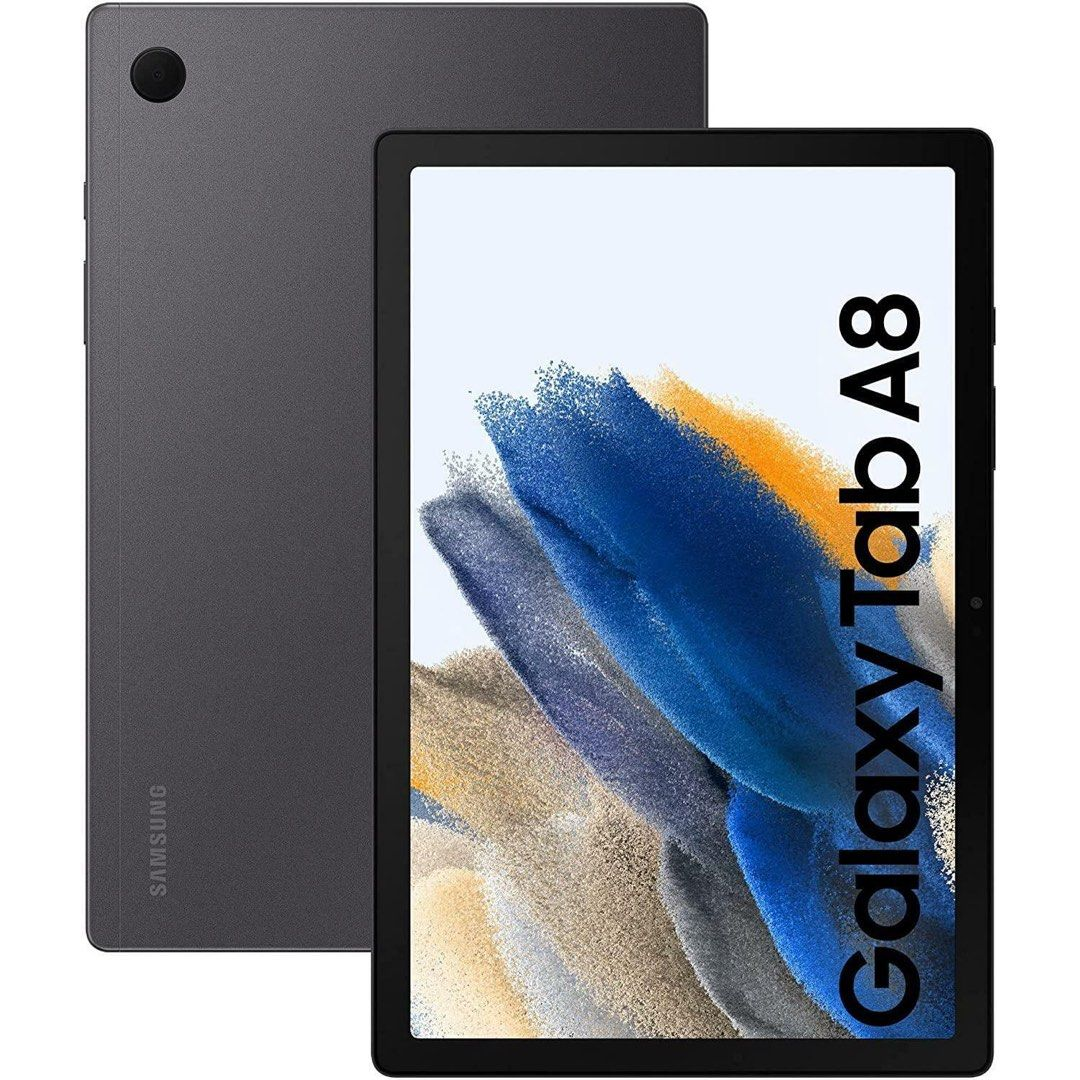
\includegraphics[width=4cm,height=4.5cm]{mainmatter/images/perantisiswa.jpg} & \multirow{5}{4cm}{Model: Samsung Galaxy Tab A8 LTE \\ Operating System: Android 14, One UI 6.0 \\ Processor: ARM Octa-Core A75 2.0GHz \\ Memory: 4GB \\ Storage: 64GB \\ Display: TFT 10.5 inches (1920 x 1200 pixel)} \\
        \cline{1-4}
        \end{tabular}
    \end{table}

    \begin{table}[htb]
        \caption{List of Software for Alunan Mobile Application} 
        \label{tab:software}
        \centering
        \begin{tabular}{|p{0.5cm}|p{3.5cm}|p{9cm}|}
        \hline
        \multicolumn{1}{|c|}{\textbf{No}} & 
        \multicolumn{1}{c|}{\textbf{Software}} & 
        \multicolumn{1}{c|}{\textbf{Descriptions}} \\
        \hline
        \multirow{1}{*}{%
            \begin{tabular}[c]{@{}p{0.5cm}@{}}
            \raggedright 1 \\
            \end{tabular}
        } &
        \multirow{1}{*}{%
            \begin{tabular}[c]{@{}p{2.5cm}@{}}
            \raggedright Figma \\
            \end{tabular}
        } &
        \multirow{1}{*}{%
            \begin{tabular}[c]{@{}p{10cm}@{}}
            \raggedright To create the user interface for the application \\
            \end{tabular}
        } \\ \hline
        \multirow{1}{*}{%
            \begin{tabular}[c]{@{}p{0.5cm}@{}}
            \raggedright 2 \\
            \end{tabular}
        } &
        \multirow{1}{*}{%
            \begin{tabular}[c]{@{}p{2.5cm}@{}}
            \raggedright Canva \\
            \end{tabular}
        } &
        \multirow{1}{*}{%
            \begin{tabular}[c]{@{}p{10cm}@{}}
            \raggedright To create a user persona for this project \\
            \end{tabular}
        } \\ \hline
        \multirow{1}{*}{%
            \begin{tabular}[c]{@{}p{0.5cm}@{}}
            \raggedright 3 \\
            \end{tabular}
        } &
        \multirow{1}{*}{%
            \begin{tabular}[c]{@{}p{2.5cm}@{}}
            \raggedright Lucidchart \\
            \end{tabular}
        } &
        \multirow{1}{*}{%
            \begin{tabular}[c]{@{}p{10cm}@{}}
            \raggedright To create a Gantt chart for the project \\
            \end{tabular}
        } \\ \hline
        \multirow{1}{*}{%
            \begin{tabular}[c]{@{}p{0.5cm}@{}}
            \raggedright 4 \\
            \end{tabular}
        } &
        \multirow{1}{*}{%
            \begin{tabular}[c]{@{}p{2.5cm}@{}}
            \raggedright Draw.io \\
            \end{tabular}
        } &
        \multirow{1}{*}{%
            \begin{tabular}[c]{@{}p{10cm}@{}}
            \raggedright To create the interaction flow for the application  \\
            \end{tabular}
        } \\ \hline
        \multirow{1}{*}{%
            \begin{tabular}[c]{@{}p{0.5cm}@{}}
            \raggedright 5 \\
            \end{tabular}
        } &
        \multirow{1}{*}{%
            \begin{tabular}[c]{@{}p{2.5cm}@{}}
            \raggedright Microsoft Word \\
            \end{tabular}
        } &
        \multirow{1}{*}{%
            \begin{tabular}[c]{@{}p{10cm}@{}}
            \raggedright To create the documentation and reports of the project \\
            \end{tabular}
        } \\ \hline
        \multirow{1}{*}{%
            \begin{tabular}[c]{@{}p{0.5cm}@{}}
            \raggedright 6 \\
            \end{tabular}
        } &
        \multirow{1}{*}{%
            \begin{tabular}[c]{@{}p{4cm}@{}}
            \raggedright Visual Studio Code \\
            \end{tabular}
        } &
        \multirow{1}{*}{%
            \begin{tabular}[c]{@{}p{10cm}@{}}
            \raggedright To create the documentation and reports of the project \\
            \end{tabular}
        } \\ \hline
        \multirow{1}{*}{%
            \begin{tabular}[c]{@{}p{0.5cm}@{}}
            \raggedright 7 \\
            \end{tabular}
        } &
        \multirow{1}{*}{%
            \begin{tabular}[c]{@{}p{2.5cm}@{}}
            \raggedright VS Code \\
            \end{tabular}
        } &
        \multirow{1}{*}{%
            \begin{tabular}[c]{@{}p{10cm}@{}}
            \raggedright To develop the front-end and back-end of the application \\
            \end{tabular}
        } \\ \hline
        \multirow{1}{*}{%
            \begin{tabular}[c]{@{}p{0.5cm}@{}}
            \raggedright 8 \\
            \end{tabular}
        } &
        \multirow{1}{*}{%
            \begin{tabular}[c]{@{}p{2.5cm}@{}}
            \raggedright phpMyAdmin \\
            \end{tabular}
        } &
        \multirow{1}{*}{%
            \begin{tabular}[c]{@{}p{10cm}@{}}
            \raggedright To develop a database of the application \\
            \end{tabular}
        } \\ \hline
        \multirow{1}{*}{%
            \begin{tabular}[c]{@{}p{0.5cm}@{}}
            \raggedright 9 \\
            \end{tabular}
        } &
        \multirow{1}{*}{%
            \begin{tabular}[c]{@{}p{2.5cm}@{}}
            \raggedright InfinityFree \\
            \end{tabular}
        } &
        \multirow{1}{*}{%
            \begin{tabular}[c]{@{}p{10cm}@{}}
            \raggedright To host the application and database \\
            \end{tabular}
        } \\ \hline
        \multirow{1}{*}{%
            \begin{tabular}[c]{@{}p{0.5cm}@{}}
            \raggedright 10 \\
            \end{tabular}
        } &
        \multirow{1}{*}{%
            \begin{tabular}[c]{@{}p{2.5cm}@{}}
            \raggedright GitHub \\
            \end{tabular}
        } &
        \multirow{1}{*}{%
            \begin{tabular}[c]{@{}p{10cm}@{}}
            \raggedright To control version of the application and report \\
            \end{tabular}
        } \\ \hline
        \end{tabular}
    \end{table} 
\end{enumerate}

\section{Designing Alunan: A Mobile Application for Local Musicians’ Online Community and Music Discovery}
This section explores the crucial structure plan required to ensure a consistent and efficient mobile application. This section also addresses Objective 2 from Chapter 1, which involves to design Alunan as a mobile application for local independent musicians’ online community and music discovery. This section includes user personas, a SCAMPER technique table, a storyboard, a flowchart, a Use Case Diagram, a Hierarchical Model, a low-fidelity prototype, and a medium-fidelity prototype. The study design and diagrams will offer a thorough overview and explanation of the project's development design.

\subsection{User Persona}
Recognizing users is the basis on which user-centered applications are built. User personas are organized depictions of the intended audience. These personas are not merely fictional characters; they are tangible archetypes that provide direction for app development in the actual world. The user persona documentation presents a range of individuals, each with unique backgrounds, objectives, and experiences. By examining their features, behaviors, and pain areas, we can determine the most effective way for the app to fulfill their demands. Figures 4.1 and 4.2 display the user personas for each user of Alunan. \\

\begin{figure}[h]
    \centering
    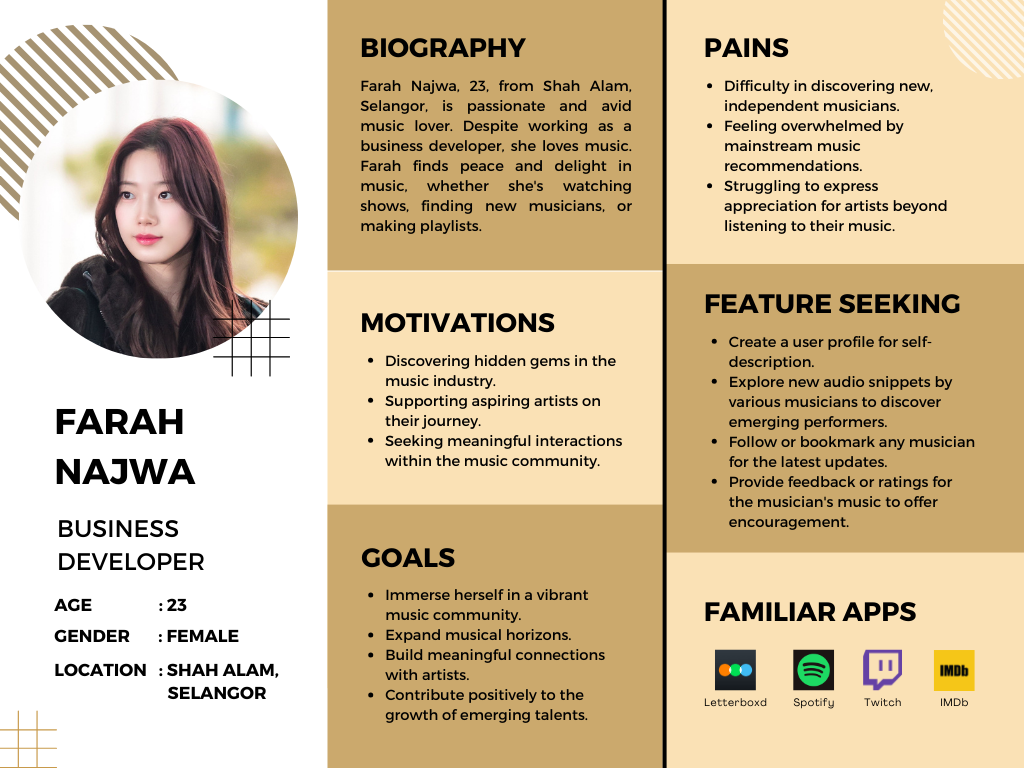
\includegraphics[width=0.9\linewidth]{mainmatter/images/userpersona1.png}
	\caption{Figure of User Persona 1 (Enthusiast)}
    \caption*{\textit{Image Source: Unsplash - Beautiful Free Images \& Pictures [https://unsplash.com/]}}
    \label{fig:myfig40}
\end{figure}

\begin{figure}[h]
    \centering
    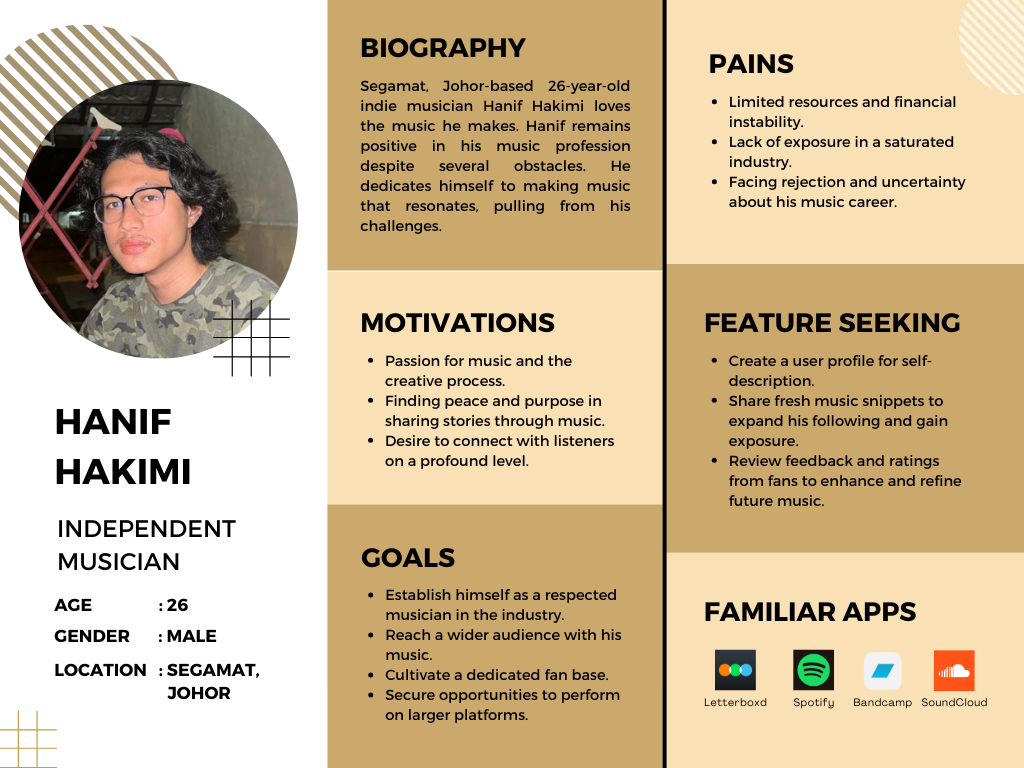
\includegraphics[width=0.9\linewidth]{mainmatter/images/userpersona2.png}
	\caption{Figure of User Persona 2 (Musician)}
    \caption*{\textit{Image Source: The image used in this persona is from a real-life person and is being consented to be used in this project.}}
    \label{fig:myfig41}
\end{figure}
\pagebreak

\subsection{SCAMPER Technique}
\textit{Purpose:} SCAMPER is a technique for looking at possible transformations that you could apply to a product or process. \parencite{santos15} Looking at these transformations can help you identify "out-of-the-box" approaches by looking at the problem from different perspectives. It is particularly useful where conventional approaches to the problem may already have been tried unsuccessfully. SCAMPER stands for: Substitute, Combine, Adapt, Modify/Magnify/Minify, Put to other uses, Eliminate, Rearrange/Reverse.
\pagebreak

\textit{Process/Product Reviewed:} Bandcamp
\begin{longtable}{|c|p{3cm}|p{4.5cm}|p{4.5cm}|}
\caption{SCAMPER Technique Table}
\label{tab:my_table}\\
\hline
\textbf{} & \textbf{Transformation} & \textbf{Typical questions} & \textbf{Solution Ideas} \\
\hline
\endfirsthead
\multicolumn{4}{c}{{\tablename\ \thetable{} -- Continued from previous page}} \\
\hline
\textbf{} & \textbf{Transformation} & \textbf{Typical questions} & \textbf{Solution Ideas} \\
\hline
\endhead

S & Substitute & What can Who: can I substitute to make an improvement? What happens if I swap X for Y? How can I substitute the place, time, materials or people? & Substitute the traditional email/password authentication with social media login options for quicker and easier access. \\
\hline
C & Combine & What materials, features, processes, people, products or components can I combine within the problem area? Where can I build synergy with other products/processes? & Combine the user profile settings and the music snippet sharing feature into a single interactive dashboard for musicians, making it more convenient for them to manage their profiles and share music snippets. \\
\hline
A & Adapt & What other products/processes are similar to the one at root cause of our problem? What if we adapted them? What could we change to make them fit our purpose? & Adapt the favorite/bookmark feature to incorporate a recommendation algorithm, suggesting musicians to enthusiasts based on their listening preferences. \\
\hline
M & Modify & What ways can we completely change the product/process? Can it be improved by making it stronger, larger, higher, longer, exaggerated or more frequent? Can it be improved by making it smaller, lighter, shorter, less prominent or less frequent? & Modify the review character limit to allow for longer, more detailed reviews, enabling enthusiasts to provide more comprehensive feedback to musicians. \\
\hline
P & Put to other uses & What other products/processes could do what we need to do? What other things are going on that we could make use of it? & Put the music ratings and reviews to other uses by aggregating data to provide insights and analytics for musicians, helping them understand audience preferences and improve their music. \\
\hline
E & Eliminate & What would happen if we remove a component of the product/process? What would happen if we remove the whole thing? How could we achieve the same objective if we weren't able to do this way? & Eliminate redundant features or options in the user interface to streamline the user experience and reduce clutter. \\
\hline
R & Rearrange & What if we reversed the process? What if we did step B before step A? What if we moved step A \& did it last step of step Z first? What if we did these two steps together? & Rearrange the layout of the 'My Reviews' page to prioritize recently reviewed posts, allowing enthusiasts to easily keep track of their recent interactions with musicians. \\
\hline
\multicolumn{4}{l}{\textit{Source: \textcite{santos15}}} \\
\end{longtable}
\pagebreak

\subsection{Storyboard Conception}
Creating a storyboard is a crucial stage in developing Alunan: A Mobile Application for Local Musicians’ Online Community and Music Discovery. This visual narrative is a crucial tool in the design and development process as it graphically depicts and maps out the user experience within the application. The storyboard in Figure 4.3 acts as a guide to help us visualize the application's operation, address any possible concerns, and ensure that the user experience matches Alunan's design objectives and problem statement.

\begin{figure}[h]
    \centering
    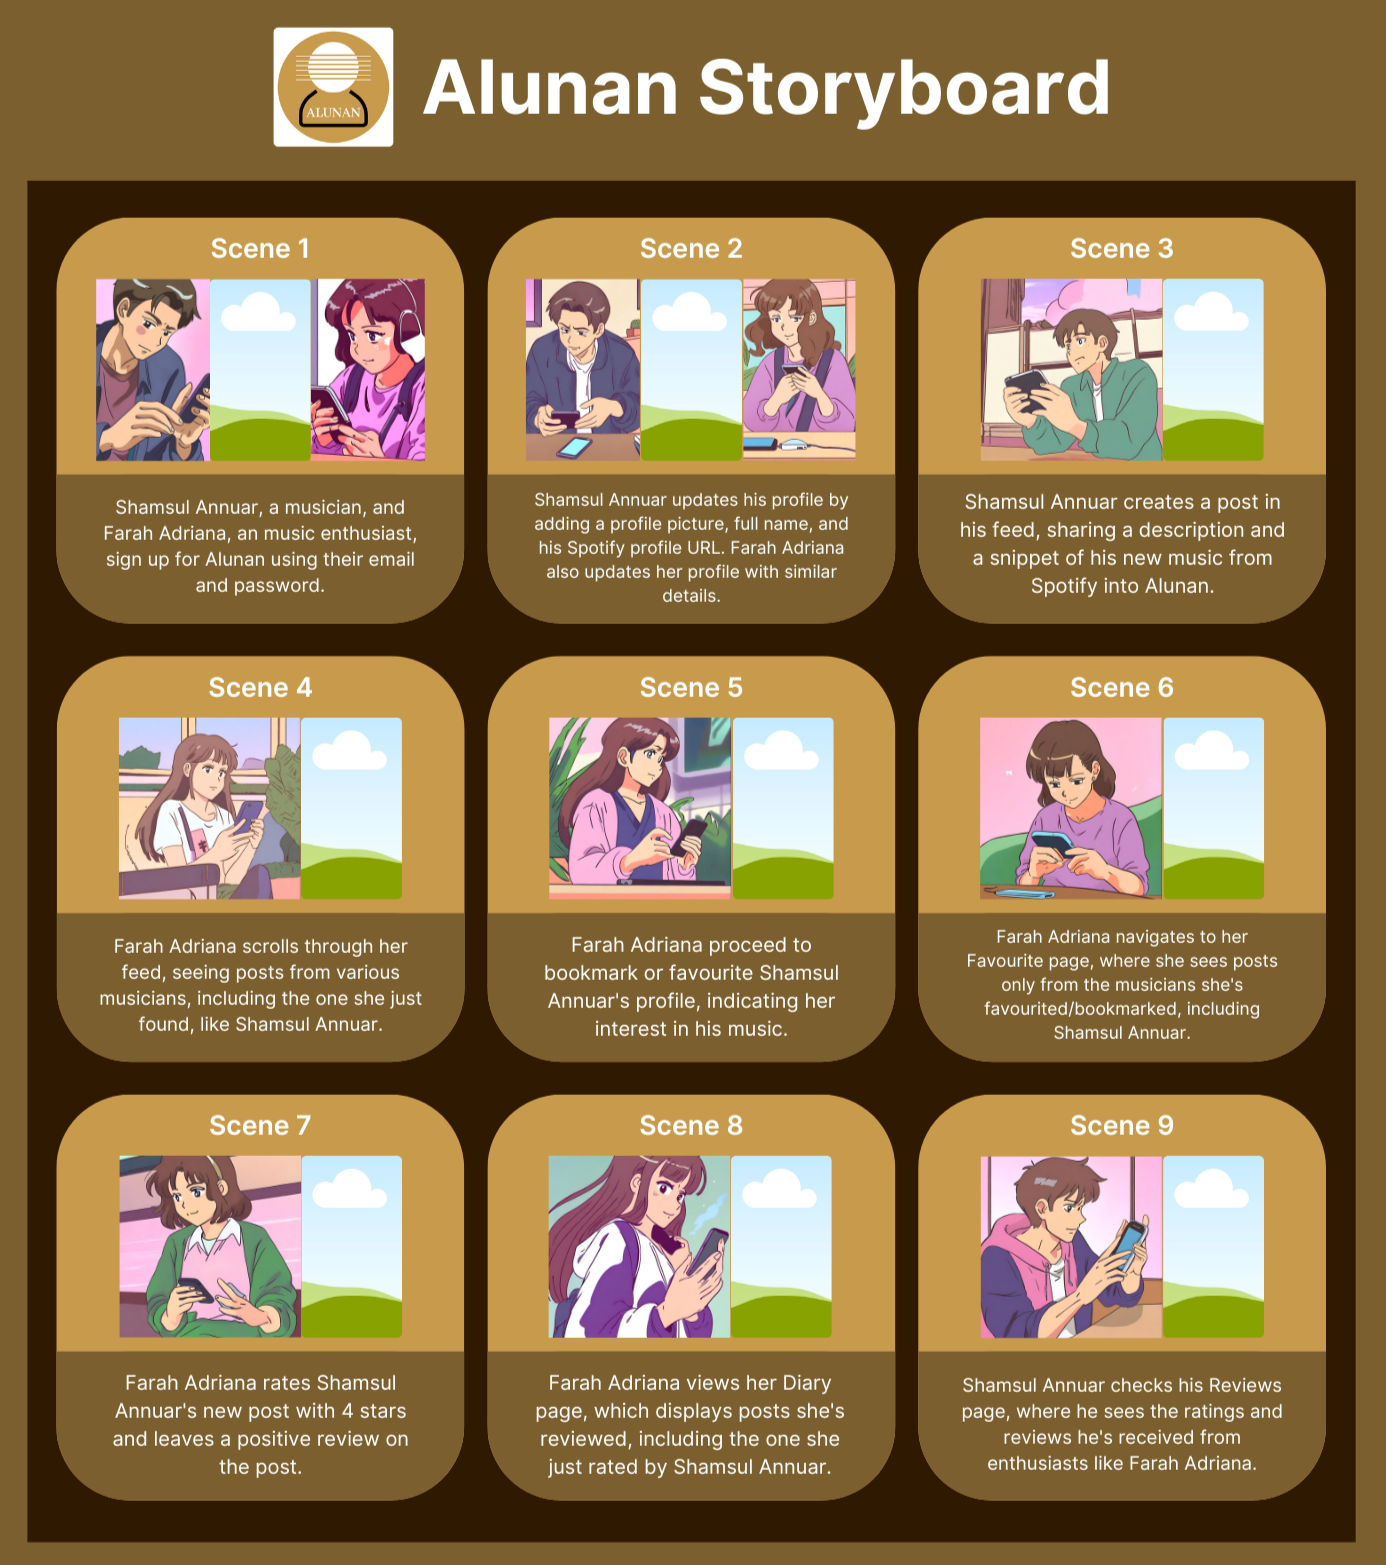
\includegraphics[width=1.0\linewidth]{mainmatter/images/storyboard.png}
	\caption{Storyboard for Alunan Mobile Application}
    \label{fig:myfig42}
\end{figure}
\pagebreak

\subsection{External Device Design Conception}
A detailed design strategy was carefully developed to integrate and implement external devices during the development of this project. External devices are essential for improving the application's capabilities, functionality, performance, and user experience. This section explained the design approach for external devices used in the development of this project.
\begin{enumerate}[A.]
    \item \textbf{IT Infra Architecture Diagram}
    \begin{figure}[h]
        \centering
        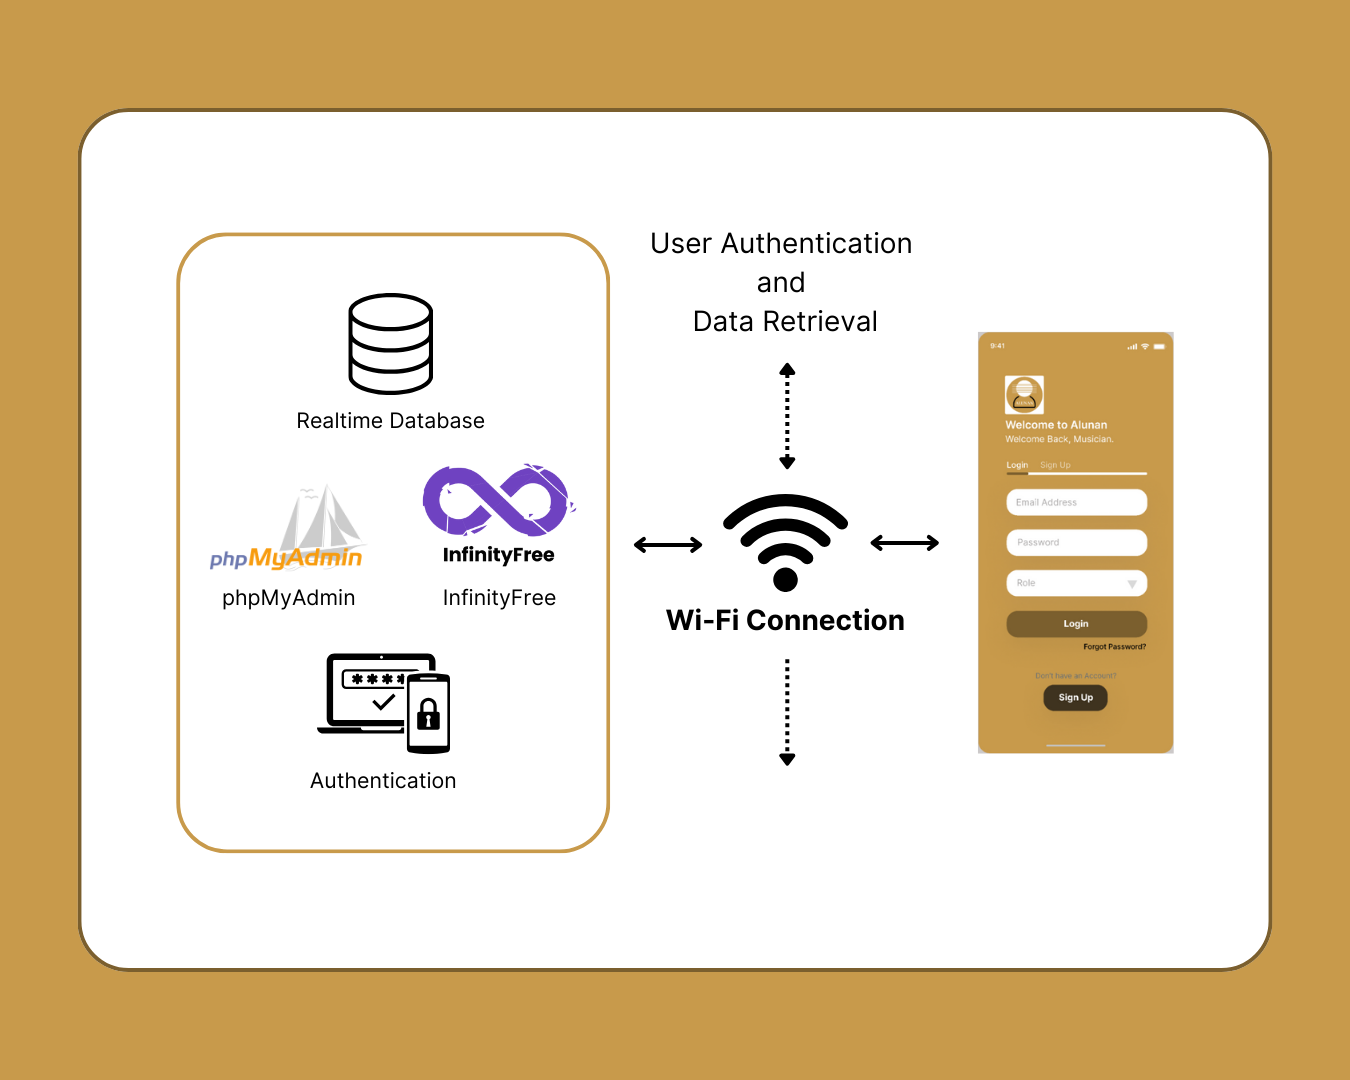
\includegraphics[width=0.7\linewidth]{mainmatter/images/itinfra.png}
        \caption{IT Infra Architecture Diagram for Alunan Mobile Application}
        \label{fig:myfig43}
    \end{figure}
\end{enumerate}

\subsection{Flowchart of Alunan: A Mobile Application for Local Musicians’ Online Community and Music Discovery}
Figure 4.5 illustrates the flowchart for Alunan, a mobile application designed for local musicians' online community and music discovery. This visual representation is crucial in developing an in-depth overview. Flowcharts are extremely helpful tools since they visually depict the sequential actions and decision points of a system. A flowchart is used to visually represent the sequence of system operations (business logic) and the criteria for employing the system functions (business rules) through a graphical picture. This flowchart, tailored for the Alunan mobile application, is crucial for illustrating the various logical steps of this application. \pagebreak
\begin{figure}[h]
    \centering
    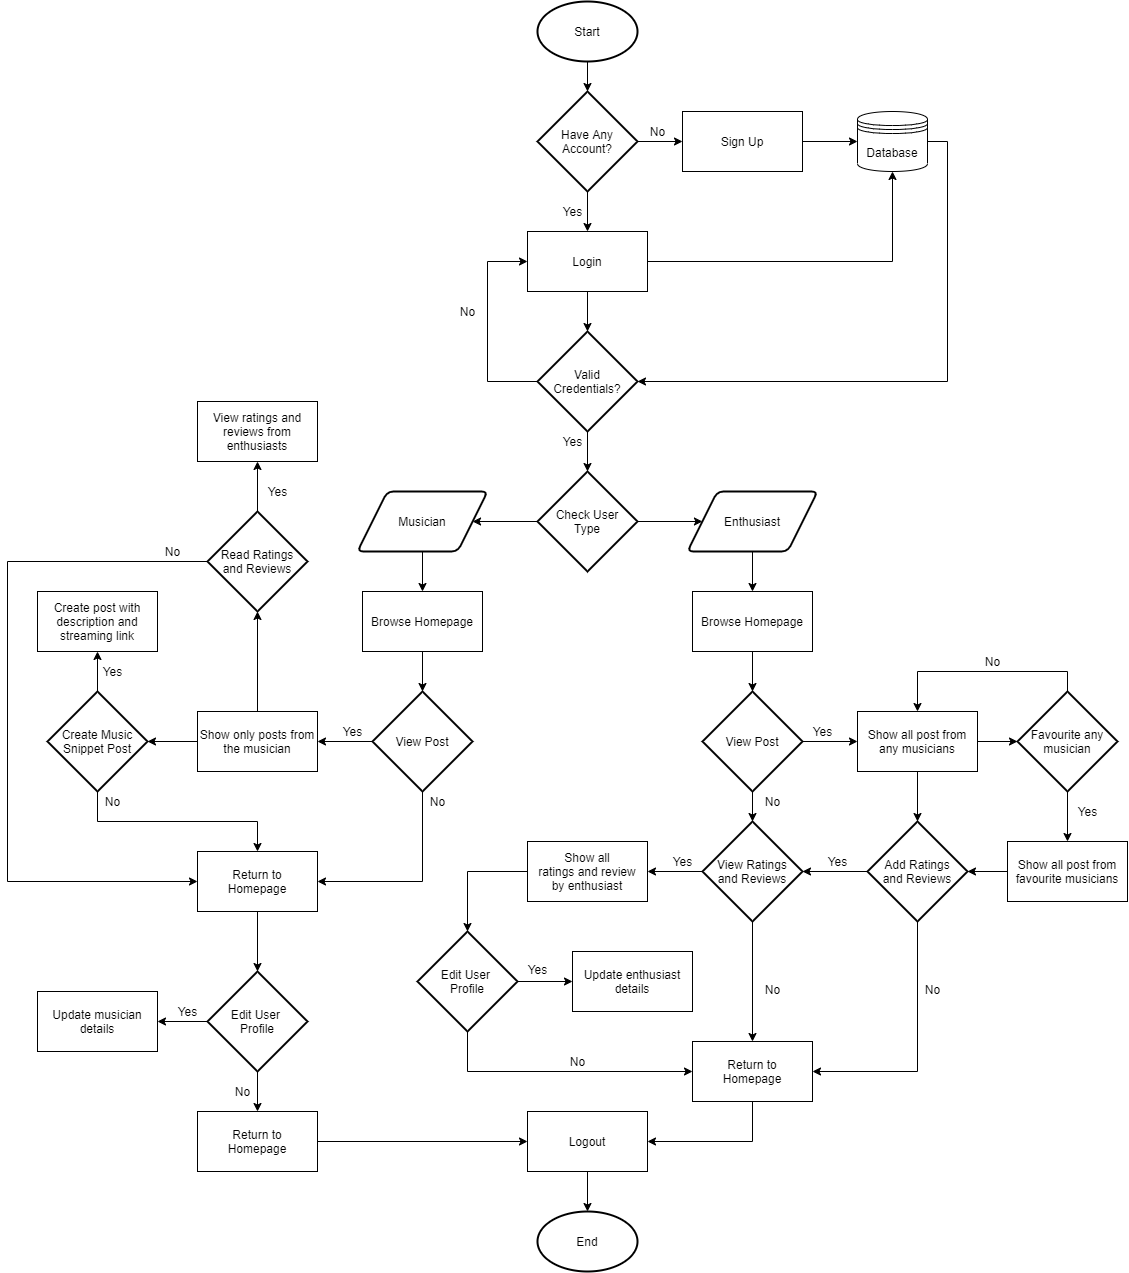
\includegraphics[width=1.0\linewidth]{mainmatter/images/flowchart.png}
    \caption{Flowchart for Alunan Mobile Application}
    \label{fig:myfig44}
\end{figure} \\
Users must sign in to continue using the Alunan mobile application. To create an account, new users must register by providing their email address, password, and user role. There are two categories of users: Musician or Enthusiast. Upon successful login, the user will be redirected to the homepage. Users of Musician can create and see posts. Musician can see ratings and reviews from Enthusiasts. Enthusiast users can browse and provide ratings or reviews on any post by Musician. Enthusiasts can freely choose to favorite any musician they prefer. Both users can access their profile, containing their name, email, Spotify URL, and profile photo. Users can easily log out of their accounts on the homepage.
\pagebreak

\subsection{Use Case Diagram of Alunan: A Mobile Application for Local Musicians’ Online Community and Music Discovery}
\begin{figure}[h]
    \centering
    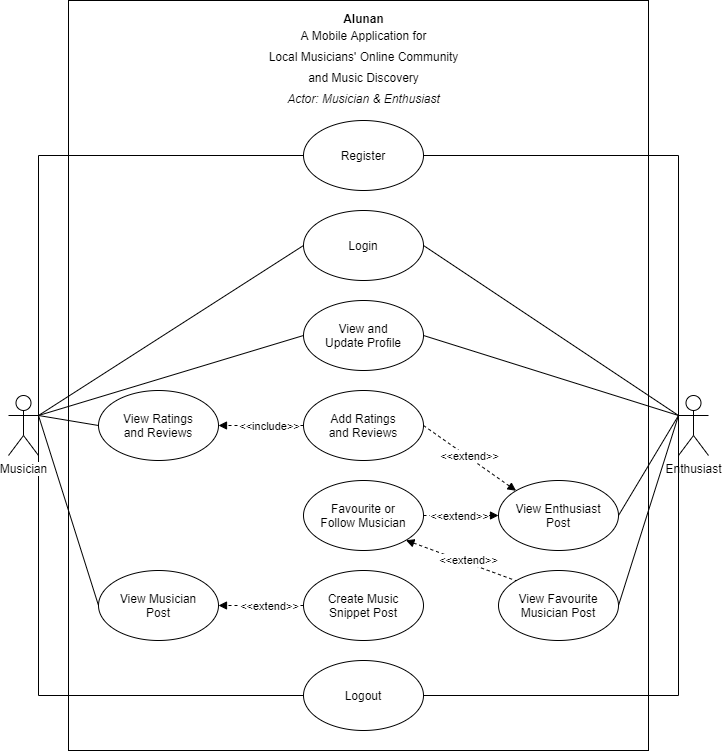
\includegraphics[width=1.0\linewidth]{mainmatter/images/usecasemain.png}
    \caption{Use Case Diagram for Alunan Mobile Application}
    \label{fig:myfig45}
\end{figure}
The use case diagram will help illustrate the interactions between the user and the system. It offers a comprehensive insight into user capabilities and how systems respond to user commands. Figure 4.6 illustrates the use case diagram, while Table 4.6 provides a summary of the use case diagram for the Alunan mobile application.
\pagebreak

\begin{table}[ht]
    \centering
    \caption{Use Case Diagram Summary for Alunan Mobile Application}
    \begin{tabular}
        {|>{\raggedright}p{2cm}|>{\raggedright}p{4cm}|>{\raggedright\arraybackslash}p{7cm}|}
    \hline
    \textbf{Actor} & \textbf{Action} & \textbf{Description} \\
    \hline
    \multirow{6}{2cm}{\vspace{-4cm}Musician} & Register & To access the Alunan mobile application features, any musician must create an account. \\
    \cline{2-3}
     & Login & Entering their email address and password allows a registered musician to log in. \\
    \cline{2-3}
     & View and Update Profile & Musicians may view and edit their profiles. \\
    \cline{2-3}
     & View Ratings and Reviews & Musicians can read reviews and ratings from their postings. They can also view ratings and reviews for other musicians. \\
    \cline{2-3}
     & View Musician Post & Musicians can access and see posts made by other musicians. In addition, they can create posts for sharing music. \\
    \cline{2-3}
     & Logout & Musicians can terminate their session on the mobile application by simply logging out. \\
    \hline
    \multirow{6}{2cm}{\vspace{-5cm}Enthusiast} & Register & Anyone who enjoys music can create an account to access Alunan's mobile application features. \\
    \cline{2-3}
     & Login & Music enthusiasts can log in by entering their email address and password after registering. \\
    \cline{2-3}
     & View and Update Profile & Music enthusiasts may view and edit their profiles. \\
    \cline{2-3}
     & View All Musician Post & Music enthusiasts can browse posts from all musicians. On each post, they have the option to submit their review and rating. They can also see reviews and ratings left by other music enthusiasts. \\
    \cline{2-3}
     & View Favourite Musician Post & Any musician can be bookmarked or followed by music enthusiasts. There's also another page where users may see all posts from only their favorite musicians. \\
    \cline{2-3}
     & Logout & Music enthusiasts only need to log out of the mobile application to end their session. \\
    \hline
    \end{tabular}
\end{table}
\pagebreak

\begin{longtable}{|p{3cm}|p{5cm}|p{5cm}|}
    \caption{System Behavior Summary for Register Use Case (Musician)} \\
    \hline
    \textbf{Use Case Name:} & \multicolumn{2}{l|}{Register as Musician} \\ \hline
    \textbf{Actor:} & \multicolumn{2}{l|}{Musician} \\ \hline
    \textbf{Use Case:} & \multicolumn{2}{l|}{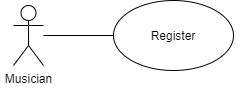
\includegraphics[width=0.5\linewidth]{mainmatter/images/sucd1.png}} \\ \hline
    \textbf{Preconditions:} & \multicolumn{2}{p{10cm}|}{Musician does not have any account yet.} \\ \hline
    \textbf{Postconditions:} & \multicolumn{2}{p{10cm}|}{Musician account created.} \\ \hline
    \multirow{5}{3cm}{\raggedright \textbf{Flow of the event:}} & \textbf{Actor} & \textbf{Application} \\ \cline{2-3}
    & 1. The system displays the Sign-Up page. & 1. The application verifies user details. \\ \cline{2-3}
    & 2. Users enter full name, email address, password, and role as Musician. & 2. The application creates the account.  \\ \cline{2-3}
    & 3. Users submit entered details. & 3. The application notifies the musician that the account has been created.  \\ \cline{2-3}
    & 4. Use case ends. &  \\ \hline
    \multirow{2}{3cm}{\raggedright \textbf{Exceptions Flow:}} 
    & \multicolumn{2}{p{10cm}|}{\raggedright E 1.0 If the musician enters invalid account details, a display message will pop out “Invalid Data”} \\ \cline{2-3}
    & \multicolumn{2}{p{10cm}|}{\raggedright E 2.0 If the musician enters an email that already exists, A display message will pop out “Email already registered.”} \\ \hline
\end{longtable}
\pagebreak

\begin{longtable}{|p{3cm}|p{5cm}|p{5cm}|}
    \caption{System Behavior Summary for Login Use Case (Musician)} \\
    \hline
    \textbf{Use Case Name:} & \multicolumn{2}{l|}{Login as Musician} \\ \hline
    \textbf{Actor:} & \multicolumn{2}{l|}{Musician} \\ \hline
    \textbf{Use Case:} & \multicolumn{2}{l|}{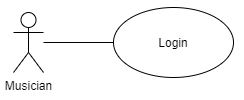
\includegraphics[width=0.5\linewidth]{mainmatter/images/sucd2.png}} \\ \hline
    \textbf{Preconditions:} & \multicolumn{2}{p{10cm}|}{Musician already created an account.} \\ \hline
    \textbf{Postconditions:} & \multicolumn{2}{p{10cm}|}{Musician logged in to the account.} \\ \hline
    \multirow{4}{3cm}{\raggedright \textbf{Flow of the event:}} & \textbf{Actor} & \textbf{Application} \\ \cline{2-3}
    & 1. The user enters details such as email address and password & 1. The system displays the login page. \\ \cline{2-3}
    & 2. The user submits the entered email address and password. & 2. The system verifies the entered email address and password. \\ \cline{2-3}
    & 3. Use case ends. & \\ \hline
    \multirow{1}{3cm}{\raggedright \textbf{Exceptions Flow:}} 
    & \multicolumn{2}{p{10cm}|}{\raggedright E 1.0 If the musician enters invalid account details, a display message will pop out “Invalid Login”} \\ \hline
\end{longtable}
\pagebreak

\begin{longtable}{|p{3cm}|p{5cm}|p{5cm}|}
    \caption{System Behavior Summary for View and Update Profile Use Case (Musician)} \\
    \hline
    \textbf{Use Case Name:} & \multicolumn{2}{l|}{View and Update Profile as Musician} \\ \hline
    \textbf{Actor:} & \multicolumn{2}{l|}{Musician} \\ \hline
    \textbf{Use Case:} & \multicolumn{2}{l|}{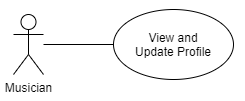
\includegraphics[width=0.5\linewidth]{mainmatter/images/sucd3.png}} \\ \hline
    \textbf{Preconditions:} & \multicolumn{2}{p{10cm}|}{Musician logged in to the account.} \\ \hline
    \textbf{Postconditions:} & \multicolumn{2}{p{10cm}|}{Musician viewed and updated profile.} \\ \hline
    \multirow{6}{3cm}{\raggedright \textbf{Flow of the event:}} & \textbf{Actor} & \textbf{Application} \\ \cline{2-3}
    & 1. The user clicked on the profile picture to access the profile page. & 1. The application displays the profile page. \\ \cline{2-3}
    & 2. The user views details such as profile picture, name, password, and Spotify URL. & 2. The application displays all the user's details.  \\ \cline{2-3}
    & 3. The user clicked on the 'Update Profile' button. & 3. The application redirects to the updated profile page.  \\ \cline{2-3}
    & 4. The user can update any of the profile details and click on the 'Save Changes' button. & 4. The application redirects back to the profile page. \\ \cline{2-3}
    & 5. Use case ends. & \\ \hline
    \multirow{2}{3cm}{\raggedright \textbf{Exceptions Flow:}} & \multicolumn{2}{p{10cm}|}{\raggedright E 1.0 If the musician chooses an invalid type of file for a picture, a display message will pop out “Invalid Picture File”.} \\ \cline{2-3}
    & \multicolumn{2}{p{10cm}|}{\raggedright E 2.0 If the musician removes the profile picture, the application will set a default profile picture for the user.} \\ \hline
\end{longtable}
\pagebreak

\begin{longtable}{|p{3cm}|p{5cm}|p{5cm}|}
    \caption{System Behavior Summary for View Ratings and Reviews Use Case (Musician)} \\
    \hline
    \textbf{Use Case Name:} & \multicolumn{2}{l|}{View Ratings and Reviews as Musician} \\ \hline
    \textbf{Actor:} & \multicolumn{2}{l|}{Musician} \\ \hline
    \textbf{Use Case:} & \multicolumn{2}{l|}{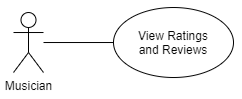
\includegraphics[width=0.5\linewidth]{mainmatter/images/sucd4.png}} \\ \hline
    \textbf{Preconditions:} & \multicolumn{2}{p{10cm}|}{Musician logged in to the account.} \\ \hline
    \textbf{Postconditions:} & \multicolumn{2}{p{10cm}|}{Musician viewed posts created by other musicians, as well as ratings and reviews by enthusiasts.} \\ \hline
    \multirow{5}{3cm}{\raggedright \textbf{Flow of the event:}} & \textbf{Actor} & \textbf{Application} \\ \cline{2-3}
    & 1. The user clicked on the 'Feed' button on the home page. & 1. The application displays all the posts from other musicians. \\ \cline{2-3}
    & 2. The user clicks on any post. & 2. The application displays the post page with the ratings and reviews submitted by the enthusiasts.  \\ \cline{2-3}
    & 3. The user can click on the Spotify URL written in the description of the post. & 3. The application will redirect to the Spotify application to play the music. \\ \cline{2-3}
    & 4. Use case ends. & \\ \hline
    \multirow{1}{3cm}{\raggedright \textbf{Exceptions Flow:}} & \multicolumn{2}{p{10cm}|}{\raggedright E 1.0 The musician can use the search bar to search for any other specific musicians.} \\ \hline
\end{longtable}
\pagebreak

\begin{longtable}{|p{3cm}|p{5cm}|p{5cm}|}
    \caption{System Behavior Summary for View Musician Post Use Case (Musician)} \\
    \hline
    \textbf{Use Case Name:} & \multicolumn{2}{l|}{View Musician Post as Musician} \\ \hline
    \textbf{Actor:} & \multicolumn{2}{l|}{Musician} \\ \hline
    \textbf{Use Case:} & \multicolumn{2}{l|}{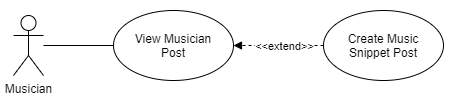
\includegraphics[width=0.5\linewidth]{mainmatter/images/sucd5.png}} \\ \hline
    \textbf{Preconditions:} & \multicolumn{2}{p{10cm}|}{Musician logged in to the account.} \\ \hline
    \textbf{Postconditions:} & \multicolumn{2}{p{10cm}|}{Musicians viewed their own posts and can create their posts.} \\ \hline
    \multirow{5}{3cm}{\raggedright \textbf{Flow of the event:}} & \textbf{Actor} & \textbf{Application} \\ \cline{2-3}
    & 1. The user clicked on the 'My Post' button on the home page. & 1. The application displays all the posts only by the musician. \\ \cline{2-3}
    & 2. The user clicks on any post. & 2. The application displays the post page with the ratings and reviews submitted by the enthusiasts. \\ \cline{2-3}
    & 3. The user can also edit or delete the post. & 3. The application updates or deletes the post selected by the user.  \\ \cline{2-3}
    & 4. Use case ends. &  \\ \hline
    \multirow{1}{3cm}{\raggedright \textbf{Exceptions Flow:}} & \multicolumn{2}{p{10cm}|}{\raggedright E 1.0 The musician can create a new post by clicking on the 'Add Post' button.} \\ \hline
\end{longtable}
\pagebreak

\begin{longtable}{|p{3cm}|p{5cm}|p{5cm}|}
    \caption{System Behavior Summary for Logout Use Case (Musician)} \\
    \hline
    \textbf{Use Case Name:} & \multicolumn{2}{l|}{Logout as Musician} \\ \hline
    \textbf{Actor:} & \multicolumn{2}{l|}{Musician} \\ \hline
    \textbf{Use Case:} & \multicolumn{2}{l|}{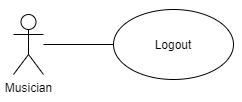
\includegraphics[width=0.5\linewidth]{mainmatter/images/sucd6.png}} \\ \hline
    \textbf{Preconditions:} & \multicolumn{2}{p{10cm}|}{Musician logged in to the account.} \\ \hline
    \textbf{Postconditions:} & \multicolumn{2}{p{10cm}|}{Musician logged out of the account.} \\ \hline
    \multirow{4}{3cm}{\raggedright \textbf{Flow of the event:}} & \textbf{Actor} & \textbf{Application} \\ \cline{2-3}
    & 1. The user clicks on the logout button on the main page. & 1. The application displays the logout page. \\ \cline{2-3}
    & 2. The user clicks again on the logout button to confirm the process. & 2. The application ends the session and logs the user out.  \\ \cline{2-3}
    & 3. Use case ends. &  \\ \hline
    \multirow{2}{3cm}{\raggedright \textbf{Exceptions Flow:}} & \multicolumn{2}{p{10cm}|}{\raggedright E 1.0 If the musician clicks on the 'Cancel' button, it will redirect back to the main page.} \\ \cline{2-3}
    & \multicolumn{2}{p{10cm}|}{\raggedright E 2.0 If the musician already logged out, it will redirect back to the login page.} \\ \hline
\end{longtable}
\pagebreak

\begin{longtable}{|p{3cm}|p{5cm}|p{5cm}|}
    \caption{System Behavior Summary for Register Use Case (Enthusiast)} \\
    \hline
    \textbf{Use Case Name:} & \multicolumn{2}{l|}{Register as Enthusiast} \\ \hline
    \textbf{Actor:} & \multicolumn{2}{l|}{Enthusiast} \\ \hline
    \textbf{Use Case:} & \multicolumn{2}{l|}{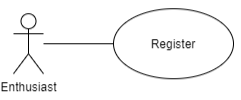
\includegraphics[width=0.5\linewidth]{mainmatter/images/sucd7.png}} \\ \hline
    \textbf{Preconditions:} & \multicolumn{2}{p{10cm}|}{Enthusiast does not have any account yet.} \\ \hline
    \textbf{Postconditions:} & \multicolumn{2}{p{10cm}|}{Enthusiast account created.} \\ \hline
    \multirow{5}{3cm}{\raggedright \textbf{Flow of the event:}} & \textbf{Actor} & \textbf{Application} \\ \cline{2-3}
    & 1. The system displays the Sign-Up page. & 1. The application verifies user details. \\ \cline{2-3}
    & 2. Users enter their full name, email address, password, and role as Enthusiast. & 2. The application creates the account.  \\ \cline{2-3}
    & 3. Users submit entered details. & 3. The application notifies the enthusiast that the account has been created.  \\ \cline{2-3}
    & 4. Use case ends. &  \\ \hline
    \multirow{2}{3cm}{\raggedright \textbf{Exceptions Flow:}} 
    & \multicolumn{2}{p{10cm}|}{\raggedright E 1.0 If the enthusiast enters invalid account details, a display message will pop out “Invalid Data”} \\ \cline{2-3}
    & \multicolumn{2}{p{10cm}|}{\raggedright E 2.0 If the enthusiast enters an email that already exists, A display message will pop out “Email already registered.”} \\ \hline
\end{longtable}
\pagebreak

\begin{longtable}{|p{3cm}|p{5cm}|p{5cm}|}
    \caption{System Behavior Summary for Login Use Case (Enthusiast)} \\
    \hline
    \textbf{Use Case Name:} & \multicolumn{2}{l|}{Login as Enthusiast} \\ \hline
    \textbf{Actor:} & \multicolumn{2}{l|}{Enthusiast} \\ \hline
    \textbf{Use Case:} & \multicolumn{2}{l|}{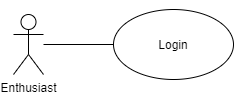
\includegraphics[width=0.5\linewidth]{mainmatter/images/sucd8.png}} \\ \hline
    \textbf{Preconditions:} & \multicolumn{2}{p{10cm}|}{Enthusiast already created an account.} \\ \hline
    \textbf{Postconditions:} & \multicolumn{2}{p{10cm}|}{Enthusiast logged in to the account.} \\ \hline
    \multirow{4}{3cm}{\raggedright \textbf{Flow of the event:}} & \textbf{Actor} & \textbf{Application} \\ \cline{2-3}
    & 1. The user enters details such as email address and password & 1. The system displays the login page. \\ \cline{2-3}
    & 2. The user submits the entered email address and password. & 2. The system verifies the entered email address and password. \\ \cline{2-3}
    & 3. Use case ends. & \\ \hline
    \multirow{1}{3cm}{\raggedright \textbf{Exceptions Flow:}} 
    & \multicolumn{2}{p{10cm}|}{\raggedright E 1.0 If the enthusiast enters invalid account details, a display message will pop out “Invalid Login”} \\ \hline
\end{longtable}
\pagebreak

\begin{longtable}{|p{3cm}|p{5cm}|p{5cm}|}
    \caption{System Behavior Summary for View and Update Profile Use Case (Enthusiast)} \\
    \hline
    \textbf{Use Case Name:} & \multicolumn{2}{l|}{View and Update Profile as Enthusiast} \\ \hline
    \textbf{Actor:} & \multicolumn{2}{l|}{Enthusiast} \\ \hline
    \textbf{Use Case:} & \multicolumn{2}{l|}{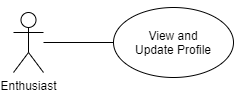
\includegraphics[width=0.5\linewidth]{mainmatter/images/sucd9.png}} \\ \hline
    \textbf{Preconditions:} & \multicolumn{2}{p{10cm}|}{Enthusiast logged in to the account.} \\ \hline
    \textbf{Postconditions:} & \multicolumn{2}{p{10cm}|}{Enthusiast viewed and updated profile.} \\ \hline
    \multirow{6}{3cm}{\raggedright \textbf{Flow of the event:}} & \textbf{Actor} & \textbf{Application} \\ \cline{2-3}
    & 1. The user clicked on the profile picture to access the profile page. & 1. The application displays the profile page. \\ \cline{2-3}
    & 2. The user views details such as profile picture, name, password, and Spotify URL. & 2. The application displays all the user's details.  \\ \cline{2-3}
    & 3. The user clicked on the 'Update Profile' button. & 3. The application redirects to the updated profile page.  \\ \cline{2-3}
    & 4. The user can update any of the profile details and click on the 'Save Changes' button. & 4. The application redirects back to the profile page. \\ \cline{2-3}
    & 5. Use case ends. & \\ \hline
    \multirow{2}{3cm}{\raggedright \textbf{Exceptions Flow:}} & \multicolumn{2}{p{10cm}|}{\raggedright E 1.0 If the enthusiast chooses an invalid type of file for a picture, a display message will pop out “Invalid Picture File”.} \\ \cline{2-3}
    & \multicolumn{2}{p{10cm}|}{\raggedright E 2.0 If the enthusiast removes the profile picture, the application will set a default profile picture for the user.} \\ \hline
\end{longtable}
\pagebreak

\begin{longtable}{|p{3cm}|p{5cm}|p{5cm}|}
    \caption{System Behavior Summary for View All Musician Post Use Case (Enthusiast)} \\
    \hline
    \textbf{Use Case Name:} & \multicolumn{2}{l|}{View All Musician Post as Enthusiast} \\ \hline
    \textbf{Actor:} & \multicolumn{2}{l|}{Enthusiast} \\ \hline
    \textbf{Use Case:} & \multicolumn{2}{l|}{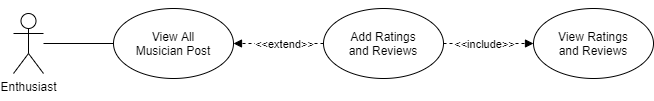
\includegraphics[width=0.5\linewidth]{mainmatter/images/sucd10.png}} \\ \hline
    \textbf{Preconditions:} & \multicolumn{2}{p{10cm}|}{Enthusiast logged in to the account.} \\ \hline
    \textbf{Postconditions:} & \multicolumn{2}{p{10cm}|}{Enthusiasts viewed all musician posts, view ratings and reviews of the post and can their own ratings and reviews.} \\ \hline
    \multirow{4}{3cm}{\raggedright \textbf{Flow of the event:}} & \textbf{Actor} & \textbf{Application} \\ \cline{2-3}
    & 1. The user views all the posts by all musicians on the 'Feed' page. & 1. The application displays all the posts created by musicians. \\ \cline{2-3}
    & 2. The user can click on any post to view ratings and reviews of the post by other enthusiasts. & 2. The application displays all the ratings and reviews by other enthusiasts.  \\ \cline{2-3}
    & 3. Use case ends. & \\ \hline
    \multirow{3}{3cm}{\raggedright \textbf{Exceptions Flow:}} & \multicolumn{2}{p{10cm}|}{\raggedright E 1.0 The enthusiast can add rating and review for the post by clicking on the 'Add Review' button.} \\ \cline{2-3}
    & \multicolumn{2}{p{10cm}|}{\raggedright E 1.1 By adding a new review, the enthusiast can also edit and delete the review created.} \\ \cline{2-3}
    & \multicolumn{2}{p{10cm}|}{\raggedright E 2.0 The enthusiast can search posts by any musician by entering any musician's name in the search bar.} \\ \hline
\end{longtable}
\pagebreak

\begin{longtable}{|p{3cm}|p{5cm}|p{5cm}|}
    \caption{System Behavior Summary for View Favourite Musician Post Use Case (Enthusiast)} \\
    \hline
    \textbf{Use Case Name:} & \multicolumn{2}{l|}{View Favourite Musician Post as Enthusiast} \\ \hline
    \textbf{Actor:} & \multicolumn{2}{l|}{Enthusiast} \\ \hline
    \textbf{Use Case:} & \multicolumn{2}{l|}{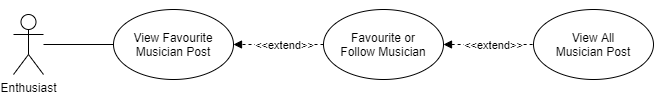
\includegraphics[width=0.5\linewidth]{mainmatter/images/sucd11.png}} \\ \hline
    \textbf{Preconditions:} & \multicolumn{2}{p{10cm}|}{Enthusiast logged in to the account.} \\ \hline
    \textbf{Postconditions:} & \multicolumn{2}{p{10cm}|}{Enthusiasts viewed favorite musician posts, favorite or follow musicians and can view all musician posts.} \\ \hline
    \multirow{6}{3cm}{\raggedright \textbf{Flow of the event:}} & \textbf{Actor} & \textbf{Application} \\ \cline{2-3}
    & 1. The user views all the posts by all musicians on the 'Feed' page. & 1. The application displays all the posts created by musicians. \\ \cline{2-3}
    & 2. The user can click on any profile picture on the post to view the musician's profile. & 2. The application displays the musician's profile.  \\ \cline{2-3}
    & 3. The user can favorite or bookmark any musician by clicking the 'bookmark' button. & 3. The application stores the bookmarked musician for the enthusiast. \\ \cline{2-3}
    & 4. The user can view all favorited musicians’ posts by clicking on the 'Favourite' button. & 4. The application displays all favorited musicians’ posts. \\ \cline{2-3}
    & 5. Use case ends. & \\ \hline
    \multirow{1}{3cm}{\raggedright \textbf{Exceptions Flow:}} & \multicolumn{2}{p{10cm}|}{\raggedright E 2.0 The enthusiast can search posts by any musician by entering any musician's name in the search bar.} \\ \hline
\end{longtable}
\pagebreak

\begin{longtable}{|p{3cm}|p{5cm}|p{5cm}|}
    \caption{System Behavior Summary for Logout Use Case (Enthusiast)} \\
    \hline
    \textbf{Use Case Name:} & \multicolumn{2}{l|}{Logout as Enthusiast} \\ \hline
    \textbf{Actor:} & \multicolumn{2}{l|}{Enthusiast} \\ \hline
    \textbf{Use Case:} & \multicolumn{2}{l|}{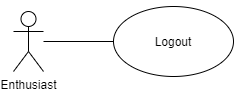
\includegraphics[width=0.5\linewidth]{mainmatter/images/sucd12.png}} \\ \hline
    \textbf{Preconditions:} & \multicolumn{2}{p{10cm}|}{Enthusiast logged in to the account.} \\ \hline
    \textbf{Postconditions:} & \multicolumn{2}{p{10cm}|}{Enthusiast logged out of the account.} \\ \hline
    \multirow{4}{3cm}{\raggedright \textbf{Flow of the event:}} & \textbf{Actor} & \textbf{Application} \\ \cline{2-3}
    & 1. The user clicks on the logout button on the main page. & 1. The application displays the logout page. \\ \cline{2-3}
    & 2. The user clicks again on the logout button to confirm the process. & 2. The application ends the session and logs the user out.  \\ \cline{2-3}
    & 3. Use case ends. &  \\ \hline
    \multirow{2}{3cm}{\raggedright \textbf{Exceptions Flow:}} & \multicolumn{2}{p{10cm}|}{\raggedright E 1.0 If the enthusiast clicks on the 'Cancel' button, it will redirect back to the main page.} \\ \cline{2-3}
    & \multicolumn{2}{p{10cm}|}{\raggedright E 2.0 If the enthusiast already logged out, it will redirect back to the login page.} \\ \hline
\end{longtable}
\pagebreak

\subsection{Data Design for Alunan: A Mobile Application for Local Musicians’ Online Community and Music Discovery}
\begin{enumerate}[A.]
    \item \textbf{Hierarchical Model Diagram}
    \begin{figure}[h]
        \centering
        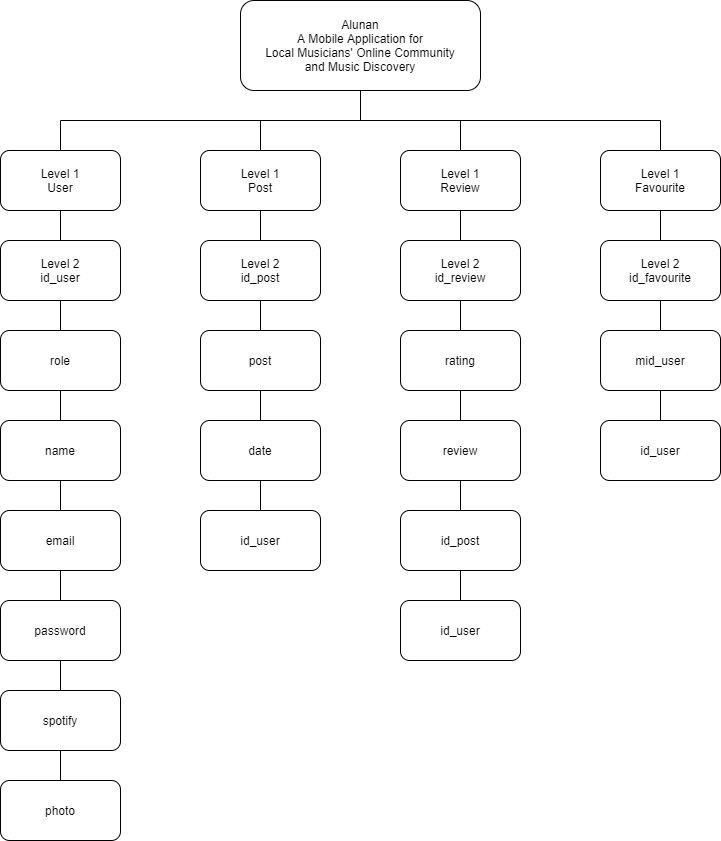
\includegraphics[width=0.9\linewidth]{mainmatter/images/hierachical.png}
        \caption{Hierarchical Model Diagram for Alunan Mobile Application}
        \label{fig:myfig46}
    \end{figure} \\
    The hierarchical diagram for the Alunan mobile application is depicted in Figure 4.7 below. It represents the overall structure of the database and provides a clear image of how data is organized in it. At the first level, key entities such as User, Post, Review, and Favourite are identified, each carrying unique forms of data. User, for example, submit information such as their role, name, email, password, Spotify profile, and photo. Furthermore, Post represent critical information such as post description, and date posted. Meanwhile, Review symbolizes the rating and review that the enthusiast submits. Lastly, Favourite represents data such as mid\_user, and id\_user, that store any musician profile that is bookmarked by the enthusiast. The second level looks into the fundamental characteristics of each object, providing a more detailed view which are id\_user, id\_post, id\_review, and id\_favourite.

    \item \textbf{Entity Relationship Diagram}
    \begin{figure}[h]
        \centering
        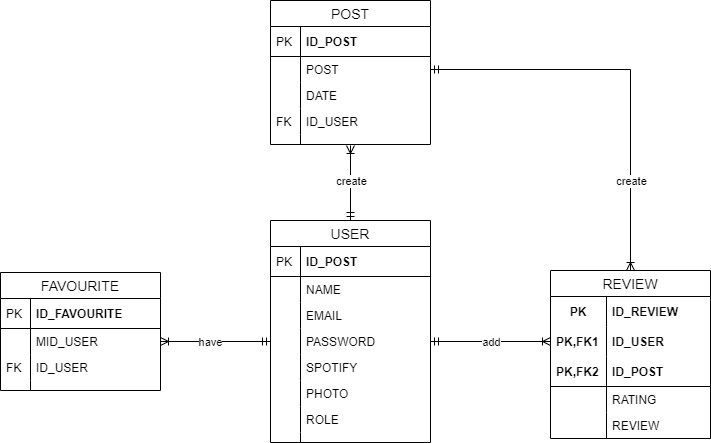
\includegraphics[width=0.9\linewidth]{mainmatter/images/erd.png}
        \caption{Entity Relationship Diagram for Alunan Mobile Application}
        \label{fig:myfig47}
    \end{figure} \\
    The ERD (Entity-Relationship Diagram) presented in Figure 4.8 shows the structure of the Alunan mobile application database, emphasizing significant entities and the relationships between them. The entities consist of USER, POST, REVIEW, and FAVOURITE. The relationships involve USERS generating POSTS and adding REVIEWS. Table 4.6 contains a data dictionary that provides a detailed description of the attributes of each table. The data dictionary specifies the contents, data types, formats, and if the attributes are necessary. It also indicates whether the attributes are primary keys (PK) or foreign keys (FK). The table captions in Table 4.7 provide a concise description of the data types utilized. This complete structure guarantees a clear and structured database architecture for effective data management within the application.
    \pagebreak
    \begin{landscape}
    \begin{longtable}
        {|>{\centering\arraybackslash}m{2.5cm}|>{\centering\arraybackslash}m{3cm}|>{\centering\arraybackslash}m{4cm}|>{\centering\arraybackslash}m{3cm}|>{\centering\arraybackslash}m{2cm}|>{\centering\arraybackslash}m{2cm}|>{\centering\arraybackslash}m{1cm}|>{\centering\arraybackslash}m{3cm}|}
        \caption{Data Dictionary for Alunan Mobile Application} \\
        \hline
        \textbf{Table Name} & \textbf{Attribute Name} & \textbf{Contents} & \textbf{Type} & \textbf{Format} & \textbf{Required} & \textbf{PK or FK} & \textbf{FK Referenced Table} \\ \hline
        \endfirsthead
        \multicolumn{8}{c}{{\tablename\ \thetable{} -- Continued from previous page}} \\
        \hline
        \textbf{Table Name} & \textbf{Attribute Name} & \textbf{Contents} & \textbf{Type} & \textbf{Format} & \textbf{Required} & \textbf{PK or FK} & \textbf{FK Referenced Table} \\ \hline
        \endhead
        \multirow{7}{*}{USER} & ID\_USER & User ID Number & INT(11) & 000000 & Y & PK & \\ \cline{2-8}
        & NAME & User Name & VARCHAR(100) & Xxxxxx & Y & & \\ \cline{2-8}
        & EMAIL & User E-Mail & VARCHAR(100) & Xxxxxx & Y & & \\ \cline{2-8}
        & PASSWORD & User Password & VARCHAR(100) & Xxxxxx & Y & & \\ \cline{2-8}
        & ROLE & User Role & VARCHAR(10) & Xxxx & Y & & \\ \cline{2-8}
        & SPOTIFY & User Spotify URL & TEXT & Xxxxxxxx & N & & \\ \cline{2-8}
        & PHOTO & User Photo & TEXT & Xxxxxxxx & N & & \\ \hline
        \multirow{5}{*}{REVIEW} & ID\_REVIEW & Review ID Number & INT(11) & 000000 & Y & PK & \\ \cline{2-8}
        & RATING & Rating from 1 to 5 & INT(11) & 000000 & Y & & \\ \cline{2-8}
        & REVIEW & Review description & TEXT & Xxxxxxxx & Y & & \\ \cline{2-8}
        & ID\_POST & Post ID Number & INT(11) & 000000 & Y & FK & POST \\ \cline{2-8}
        & ID\_USER & User ID Number & INT(11) & 000000 & Y & FK & USER \\ \hline
        \multirow{2}{*}{POST} & ID\_POST & Post ID Number & INT(11) & 000000 & Y & PK & \\ \cline{2-8}
        & POST & Post description & TEXT & Xxxxxxxx & Y & & \\ \hline
        & DATE & Post date & DATE & dd-mm-yyyy & Y & & \\ \cline{2-8}
        & ID\_USER & User ID Number & INT(11) & 000000 & Y & FK & USER \\ \hline
        \multirow{3}{*}{FAVOURITE} & ID\_FAVOURITE & Favourite ID Number & INT(11) & 000000 & Y & PK & \\ \cline{2-8}
        & MID\_USER & Musician ID Number & INT(11) & 000000 & Y & & \\ \cline{2-8}
        & ID\_USER & Enthusiast ID Number & INT(11) & 000000 & Y & FK & USER \\ \hline
    \end{longtable}

    \begin{table}[h]
        \centering
        \captionsetup{justification=centering} % Center the caption
        \caption{Table Legends for Data Dictionary}
        \begin{tabular}{|c|c|}
        \hline
        \textbf{Name} & \textbf{Description} \\
        \hline
        PK & Primary Key \\
        \hline
        FK & Foreign Key \\
        \hline
        INT & Whole numbers that range from -2,147,483,647 to 2,147,483,647 for 9 or 10 digits of precision \\
        \hline
        VARCHAR & Variable character length data (1-2,000 characters) \\
        \hline
        TEXT & Long-form text strings \\
        \hline
        DATE & Dates ranging from 1 January 100 (-657,434), to 31 December 9999 (2,958,465), and times from 0:00:00 to 23:59:59 \\
        \hline
        \end{tabular}
    \end{table}

    \end{landscape}
\end{enumerate}

\section{Developing Alunan: A Mobile Application for Local Musicians’ Online Community and Music Discovery}
\subsection{Front-End Development for Alunan: A Mobile Application for Local Musicians’ Online Community and Music Discovery}
\begin{enumerate}[1.]
    \item \textbf{Front Page}
    \item \textbf{Login \& Signup Page}
    \item \textbf{Forgot Password Page}
    \item \textbf{Information Page}
    \item \textbf{Sign Out Page}
    \item \textbf{User Profile Page (Musician \& Enthusiast)}
    \item \textbf{Update User Profile Page (Musician \& Enthusiast)}
    \item \textbf{Main Page (Musician)}
    \item \textbf{Feed Page (Musician)}
    \item \textbf{Musician Profile Page (Musician)}
    \item \textbf{Review Page (Musician)}
    \item \textbf{My Post Page (Musician)}
    \item \textbf{Edit \& Delete Post Page (Musician)}
    \item \textbf{Add Post Page (Musician)}
    \item \textbf{Main Page (Enthusiast)}
    \item \textbf{Feed Page (Enthusiast)}
    \item \textbf{Musician Profile Page (Enthusiast)}
    \item \textbf{Review Page (Enthusiast)}
    \item \textbf{Edit \& Delete Review Page (Enthusiast)}
    \item \textbf{Add Review Page (Enthusiast)}
    \item \textbf{My Review Page (Enthusiast)}
    \item \textbf{Favourite Page (Enthusiast)}
    \item \textbf{Musicians Page (Enthusiast)}
\end{enumerate}

\subsection{Back-End Development for Alunan: A Mobile Application for Local Musicians’ Online Community and Music Discovery}
\begin{enumerate}[1.]
    \item \textbf{Initialize Database}
    \item \textbf{phpMyAdmin Database (InfinityFree)}
    \item \textbf{phpMyAdmin Database (Localhost)}
    \item \textbf{File Manager (InfinityFree)}
\end{enumerate}

\subsection{System Integration}

\pagebreak

\subsection{System Testing}
\begin{enumerate}[A.]
    \item \textbf{User Testing Activities} \\
    User testing is an essential element of the product development process, aiming to collect feedback from users to improve the product's effectiveness and overall user experience. The System Usability Scale (SUS) is a widely used and efficient tool for doing user testing. The System Usability Scale (SUS) is a standardized questionnaire that is employed to assess the usability of various goods, such as websites, software programs, and physical equipment. This method is efficient and dependable for measuring customer happiness and discovering design problems in a product. \\

    User testing is performed to evaluate the acceptability and suitability of the Alunan mobile application for the online community and music discovery of local musicians. This evaluation focuses on user engagement, the effectiveness of the developed features, the application's user-friendliness, and the users' level of interest in utilizing it. Furthermore, user input can provide valuable developer insight. During the testing phase, evaluators are categorized into two groups: Musicians and Music Enthusiasts. Only individuals aged 18 or older will assess the functioning and usability of the Alunan mobile application. Once the respondents had utilized the application, they were given ten System Usability Scale (SUS) questions specifically related to the Alunan mobile application.
    \pagebreak

    \begin{figure}[h]
        \centering
        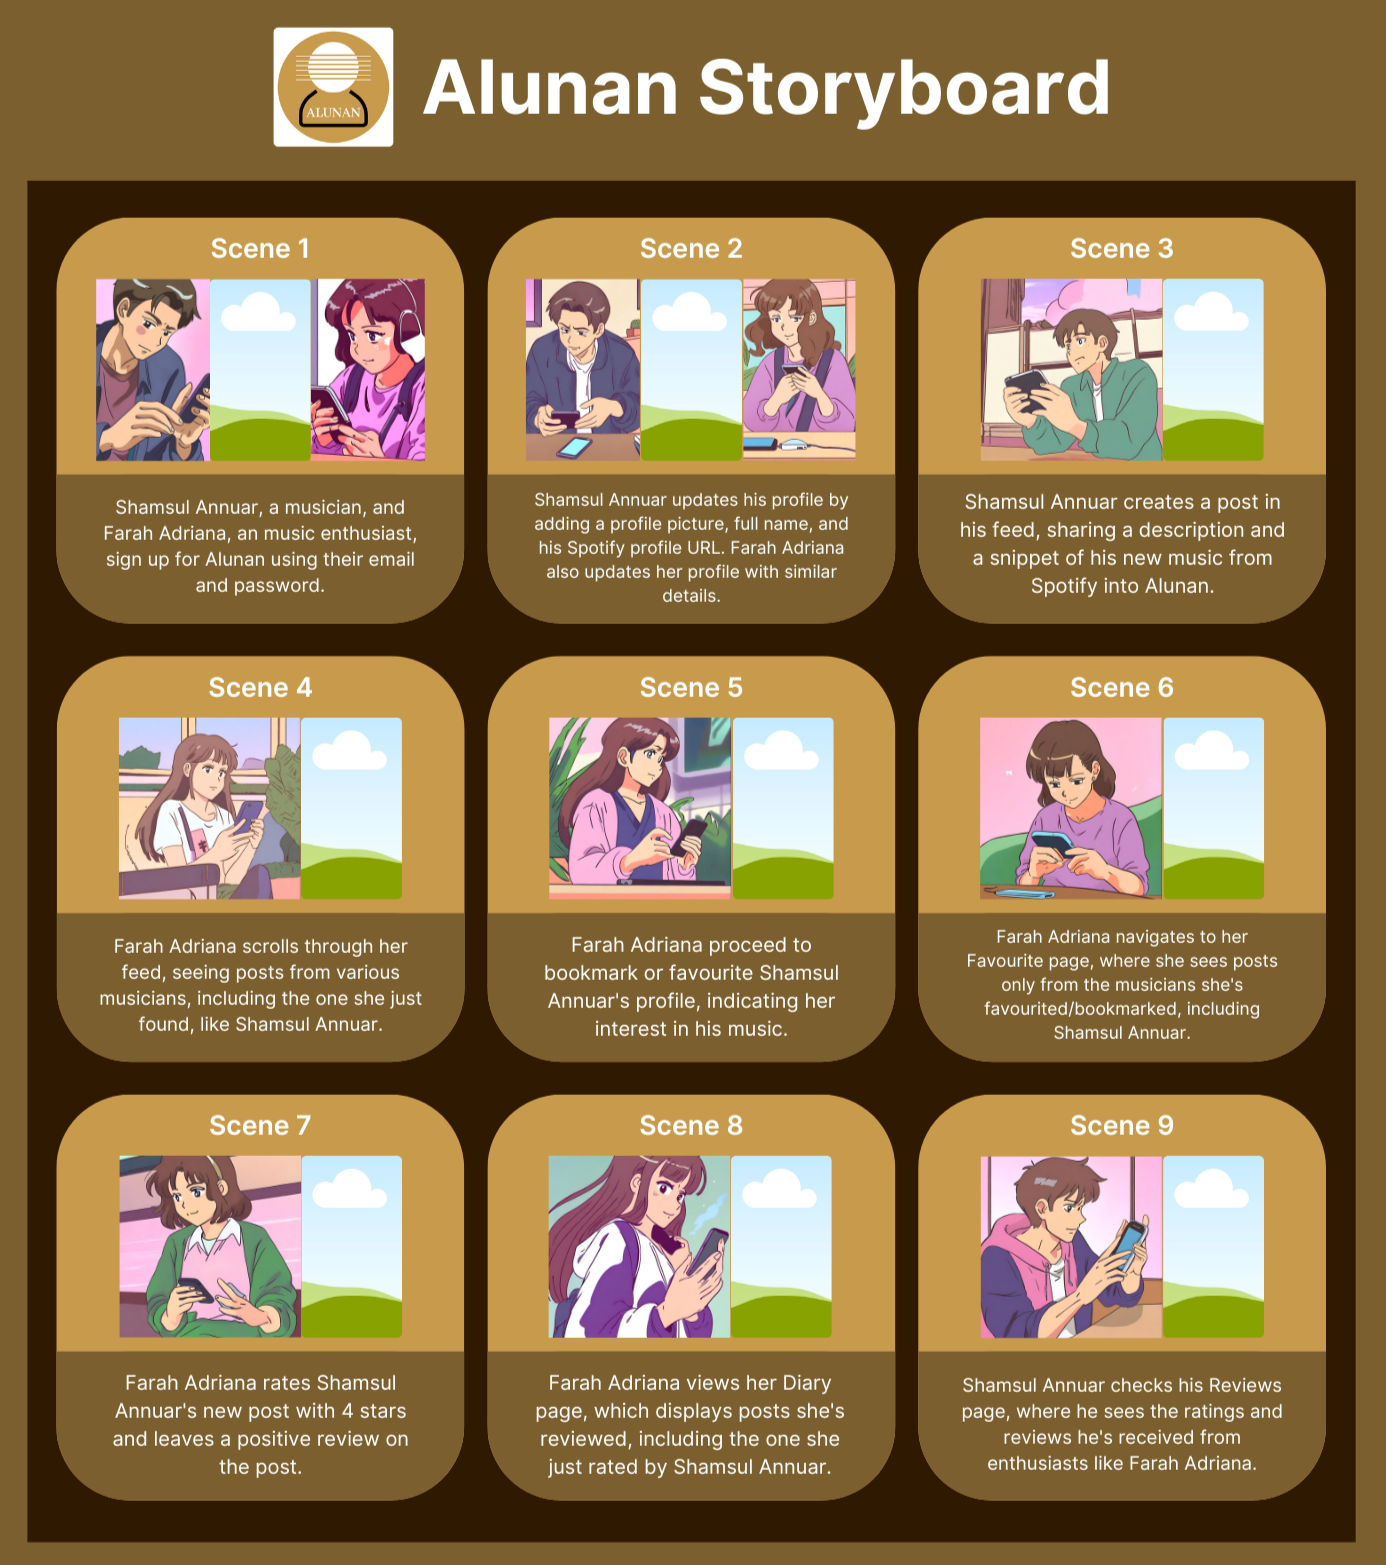
\includegraphics[width=1.0\linewidth]{mainmatter/images/storyboard.png}
        \caption{Storyboard for Alunan Mobile Application}
        \label{fig:myfig42}
    \end{figure}
    \pagebreak

    \item \textbf{User Testing Results} \\
    The Alunan mobile application will be evaluated for usability using the System Usability Scale (SUS) in this project. The SUS consists of 10 questions that evaluate usability. After the application testing was finished, around 12 users, mostly musicians and music enthusiasts, took part in SUS evaluations. Table 4.21 presents an outline of the SUS questionnaire that was given to the participants. The SUS form utilizes a scale range outlined in Table 4.22, which ranges from 1 for "Strongly Disagree" to 5 for "Strongly Agree". Table 4.23 and Table 4.24 display the findings for both Musicians and Music Enthusiasts. Furthermore, Table 4.25 displays the SUS adjective ratings assigned after calculating each user's feedback score. The form is generated using Google Forms, while the results are arranged and calculated using Google Spreadsheet. \\
    
    \begin{table}[htb]
    \caption{SUS Questionnaire for Alunan Mobile Application}
    \label{tab:mytable}
    \centering
    \begin{tabular}{|p{3cm}|p{12cm}|}
    \hline
    \multicolumn{1}{|c|}{\textbf{Number}} & 
    \multicolumn{1}{c|}{\textbf{Questionnaire}} \\
    \hline 
    \multicolumn{1}{|c|}{1} & I think that I would like to use "Alunan" application frequently \\ \hline
    \multicolumn{1}{|c|}{2} & I found "Alunan" application unnecessarily complex \\ \hline
    \multicolumn{1}{|c|}{3} & I thought "Alunan" application was easy to use \\ \hline
    \multicolumn{1}{|c|}{4} & I think that I would need the support of a technical person to be able to use "Alunan" application \\ \hline
    \multicolumn{1}{|c|}{5} & I found the various functions in "Alunan" application were well integrated \\ \hline
    \multicolumn{1}{|c|}{6} & I thought there was too much inconsistency in "Alunan" application \\ \hline
    \multicolumn{1}{|c|}{7} & I would imagine that most people would learn to use "Alunan" application very quickly \\ \hline
    \multicolumn{1}{|c|}{8} & I found "Alunan" application very cumbersome to use \\ \hline
    \multicolumn{1}{|c|}{9} & I felt very confident using "Alunan" application \\ \hline
    \multicolumn{1}{|c|}{10} & I needed to learn a lot of things before I could get going with "Alunan" application \\ \hline
    \end{tabular}
    \end{table}
    
    \begin{table}[htb]
    \caption{SUS Score Scale for Alunan Mobile Application}
    \caption*{\textit{Source: \textcite{brooke95}}} 
    \label{tab:mytable}
    \centering
    \begin{tabular}{|p{5cm}|p{10cm}|p{10cm}|p{10cm}|p{5cm}|}
    \hline
    \multicolumn{1}{|c|}{\textbf{Strongly Disagree}} & 
    \multicolumn{1}{c|}{\textbf{Disagree}} & 
    \multicolumn{1}{c|}{\textbf{Neutral}} & 
    \multicolumn{1}{c|}{\textbf{Agree}} & 
    \multicolumn{1}{c|}{\textbf{Strongly Agree}} \\
    \hline 
    \multicolumn{1}{|c|}{1} & \multicolumn{1}{c|}{2} & \multicolumn{1}{c|}{3} & \multicolumn{1}{c|}{4} & \multicolumn{1}{c|}{5}\\ \hline
    \end{tabular}
    \end{table}

    \begin{table}[h]
    \centering
    \caption{SUS Score Results (Musicians)}
    \begin{tabular}{|>{\bfseries}c|c|c|c|c|c|}
    \hline
    \textbf{Question} & \textbf{User 1} & \textbf{User 2} & \textbf{User 3} & \textbf{User 4} & \textbf{User 5} \\
    \hline
    \textbf{1} & 4 & 5 & 5 & 0 & 0 \\
    \hline
    \textbf{2} & 2 & 2 & 1 & 0 & 0 \\
    \hline
    \textbf{3} & 4 & 4 & 5 & 0 & 0 \\
    \hline
    \textbf{4} & 1 & 2 & 1 & 0 & 0 \\
    \hline
    \textbf{5} & 4 & 5 & 5 & 0 & 0 \\
    \hline
    \textbf{6} & 2 & 1 & 1 & 0 & 0 \\
    \hline
    \textbf{7} & 4 & 4 & 5 & 0 & 0 \\
    \hline
    \textbf{8} & 2 & 3 & 1 & 0 & 0 \\
    \hline
    \textbf{9} & 5 & 5 & 5 & 0 & 0 \\
    \hline
    \textbf{10} & 1 & 1 & 1 & 0 & 0 \\
    \hline
    \textbf{\parbox[c]{5cm}{\vspace{0.2cm}X = (Sum of Odd Numbered \\Questions) - 5 \vspace{0.2cm}}} & 21-5=16 & 23-5=18 & 25-5=20 & 20-5=0 & 20-5=0 \\
    \hline
    \textbf{\parbox[c]{5cm}{\vspace{0.2cm}Y = 25 - (Sum of Even \\Numbered Questions) \vspace{0.2cm}}} & 25-8=17 & 25-9=16 & 25-5=20 & 25-0=0 & 25-0=0 \\
    \hline
    \textbf{\parbox[c]{5cm}{\vspace{0.2cm}SUS Score = (X + Y) x 2.5 \vspace{0.2cm}}} & 82.5 & 85 & 100 & 0 & 0 \\
    \hline
    \end{tabular}
    \end{table}
    
    \begin{table}[h]
    \centering
    \caption{SUS Score Results (Music Enthusiasts)}
    \begin{tabular}{|>{\bfseries}c|c|c|c|c|c|}
    \hline
    \textbf{Question} & \textbf{User 1} & \textbf{User 2} & \textbf{User 3} & \textbf{User 4} & \textbf{User 5} \\
    \hline
    \textbf{1} & 4 & 0 & 0 & 0 & 0 \\
    \hline
    \textbf{2} & 2 & 0 & 0 & 0 & 0 \\
    \hline
    \textbf{3} & 4 & 0 & 0 & 0 & 0 \\
    \hline
    \textbf{4} & 2 & 0 & 0 & 0 & 0 \\
    \hline
    \textbf{5} & 4 & 0 & 0 & 0 & 0 \\
    \hline
    \textbf{6} & 2 & 0 & 0 & 0 & 0 \\
    \hline
    \textbf{7} & 4 & 0 & 0 & 0 & 0 \\
    \hline
    \textbf{8} & 2 & 0 & 0 & 0 & 0 \\
    \hline
    \textbf{9} & 4 & 0 & 0 & 0 & 0 \\
    \hline
    \textbf{10} & 2 & 0 & 0 & 0 & 0 \\
    \hline
    \textbf{\parbox[c]{5cm}{\vspace{0.2cm}X = (Sum of Odd Numbered \\Questions) - 5 \vspace{0.2cm}}} & 20-5=15 & 20-5=0 & 20-5=0 & 20-5=0 & 20-5=0 \\
    \hline
    \textbf{\parbox[c]{5cm}{\vspace{0.2cm}Y = 25 - (Sum of Even \\Numbered Questions) \vspace{0.2cm}}} & 25-10=15 & 25-0=0 & 25-0=0 & 25-0=0 & 25-0=0 \\
    \hline
    \textbf{\parbox[c]{5cm}{\vspace{0.2cm}SUS Score = (X + Y) x 2.5 \vspace{0.2cm}}} & 75 & 0 & 0 & 0 & 0 \\
    \hline
    \end{tabular}
    \end{table}

    \clearpage

    \begin{table}[h]
    \centering
    \caption{General Guideline for SUS Adjective Rating}
    \begin{tabular}{|c|c|c|}
    \hline
    \textbf{SUS Score} & \textbf{Grade} & \textbf{Adjective Rating} \\
    \hline
    $>$ 80.3 & A & Excellent \\
    \hline
    68 - 80.2 & B & Good \\
    \hline
    67 & C & Okay \\
    \hline
    51 - 66 & D & Poor \\
    \hline
    $<$ 51 & F & Awful \\
    \hline
    \end{tabular}
    \end{table}

    Based on the data provided in both Table 4.23 and Table 4.24, the SUS Score Results show positive feedback for the Alunan mobile application. The System Usability Scale (SUS) test produced an average score of 00.0, suggesting that participants held a positive perception of the product's effectiveness. The score surpasses the average SUS score of around 68, suggesting that users' experiences with the mobile application were generally favorable. Every participant offered individual input, with a significant number of them highlighting the smooth integration and user-friendly aspect of the interface. Although certain areas for enhancement were identified, participants generally reported contentment with the application's usefulness. The results are particularly promising, as they demonstrate that the system is on track to fulfill user expectations and requirements. These data indicate that users are experiencing enjoyment while using the Alunan mobile application, which implies exciting possibilities for future enhancements.
\end{enumerate}